\documentclass{article}
\usepackage{geometry}
\usepackage{hyperref}
\usepackage{fancyhdr}  
\usepackage{graphicx}

\geometry{
  top=1in,
  bottom=1.5in,
  left=1.25in,
  right=1.25in
}

\title{Rapport de projet IA41 - Rasende Roboter}
\author{SENGEL Noé, POURCINE Mattéo, FLEURET Gabriel}
\date{\today}


\begin{document}

\maketitle

\tableofcontents
\newpage
\section{Mise en contexte}
Le but de ce projet est de mettre en application les différents algorithmes vu en cours pendant le semestre d'automne 2023 en \textbf{IA41} (\href{https://fr.wikipedia.org/wiki/Algorithme_de_parcours_en_largeur}{Breadth-First Search}, \href
{	https://en.wikipedia.org/wiki/A*_search_algorithm}{A*}, \href{https://en.wikipedia.org/wiki/Depth-first_search}{Depth-first search}).\\
Ces algorithmes vont être appliqués sur un jeu de société allemand, \href{https://fr.wikipedia.org/wiki/Ricochet_Robots}{\textbf{Rasende Roboter}} ou \href{https://fr.wikipedia.org/wiki/Ricochet_Robots}{Ricochet Robots} en français, créé en 1999 par \href{https://fr.wikipedia.org/wiki/Alex_Randolph}{Alex Randolph}.\\
\\
Nous étions trois à réaliser ce projet. Pour nous permettre de s'organiser au mieux, nous avons choisit de faire un répertoire \href{https://github.com/Glenrunc/IA41_Rasende_Roboter}{\textbf {Github}}. Notre raisonnement a été assez simple concernant l'approche du projet. Nous avons décidé d'implémenter premièrement le jeu pour ensuite y incorporer les algorithmes de résolution.\\\\
Plusieurs sources ont été utiles à la réalisation de ces travaux. Vous les trouverez en fin de rapport. Pour la suite du rapport, "Intelligence artificielle" sera remplacée par "IA".
\section{Implémentation du jeu}
Nous avons fait le choix de prendre la première version du jeu. En effet une autre est apparu en 2003, qui ajoutait un robot noir, une case mission multicolore et des agencements de mur différents.
\subsection{Règles du jeu}
Les règles sont assez simple. Le joueur dispose d'un plateau de 16x16 cases. Sur celui-ci est diposé 4 robots de couleurs différentes (rouge, vert, bleu et jaune) et des jetons "missions". Une case centrale permet d'afficher la mission a atteindre par le robot de la couleur de celle-ci.\\ Le but est pour le joueur d'atteindre la mission avec le robot de la couleur correspondante en un minimum de coup et un minimum de temps. Pour cela il peut déplacer tous les robots comme il le souhaite.\\\\
\begin{figure}[h]
  \centering  
  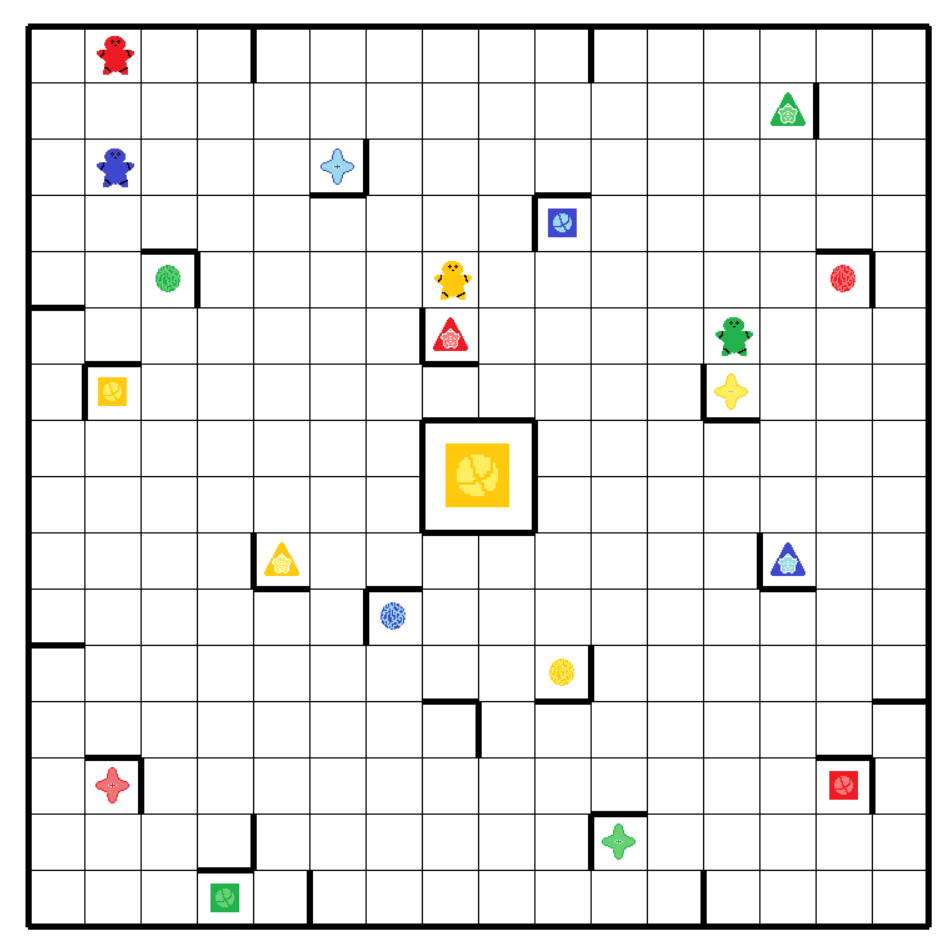
\includegraphics[width=0.5\textwidth]{map_rasende.png}  
  \caption{Image du plateau de jeu "Rasende Roboter"} 
  \label{fig:Plateau}  
\end{figure}
\\
Les déplacements sont assez simple également. Les robots ne peuvent suivre que 4 directions (haut, bas, gauche, droite). De plus une fois qu'une direction est prise, le robot en question ne s'arrête que lorsqu'il croise un mur ou un autre robot.\\\\Chaque partie commence par le tirage d'une mission. Une fois la mission choisit, un compte à rebourt est lancé. Pendant ce temps les différents joueurs analyse la position de chaque robot et essaye, dans leur tête, de trouver un moyen de résoudre le problème. Pour faciliter la compréhension, si on regarde la Figure 1, le robot jaune doit atteindre la cible afficher au centre du plateau. Ici elle se situe aux coordonnées (7,2).\\\\
Si un joueur à une solution, il fait signe et donne sa réponse. Si elle est bonne, il gagne, sinon les autres tentent de résoudre le problème.
\subsection{Choix et explications de notre implémentation}
Le but du projet étant d'implémenter différents algorithmes de résolutions, il nous ait paru évident de modifier certains points du jeu.\\\\Dans la version physique, le jeu se joue à plusieurs, chacun pour soi. Nous avons décider que notre jeu pouvait se jouer seul ou à plusieurs contre les algorithmes de résolutions. Ainsi le but de chaque partie est de résoudre le problème en moins de coup possible certes, mais surtout en moins de coup que ces algorithmes.\\\\Lorsque qu'on arrive sur le jeu, on peut choisir la difficulté de l'IA (easy, medium, hardcore).\\\\On peut également choisir de "Reset" la manche si on voit que l'on bloque. Un mode revisionnage à été implémenté pour voir les coups effectués par l'IA. Ce mode est uniquement disponible lorsque la manche est terminée et que l'IA a trouvé une solution.\\\\
Au niveau de l'ergonomie de jeu. Il se joue uniquement grâce à une souris ou un pavé tactile. Lorsque l'on clique sur un robot, un chemin s'affiche pour aider le joueur à voir les cases atteignables. Ensuite il peu cliquer sur les différents chemin possible pour déplacer le robot. 
\begin{figure}[h]
  \centering  
  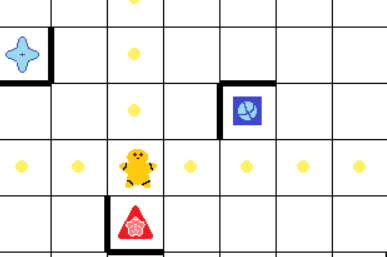
\includegraphics[width=0.5\textwidth]{deplacement.png}  
  \caption{Exemple de déplacement du robot jaune} 
  \label{fig:Plateau}  
\end{figure}\\
Pour ce qui est de l'implémentation du jeu uniquement, nous vous détailleront certaines méthodes dans la partie réservée aux algorithmes de résolution. Mais pour le reste, nous avons décidé de faire uniquement un diagramme de classe pour rendre plus visuel nos explications.
\begin{figure}
  \centering  
  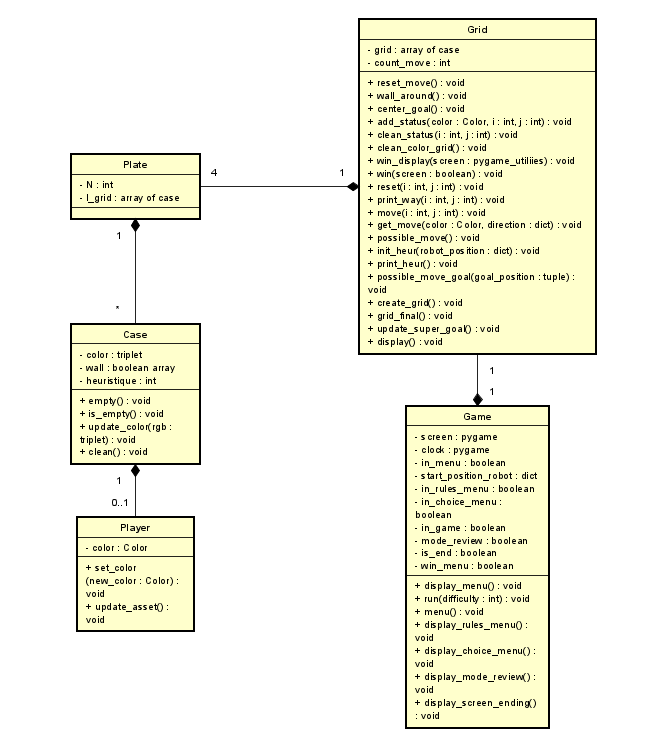
\includegraphics[width=1\textwidth]{diagram_class.png}  
  \caption{Diagramme de classe du jeu Rasende Roboter} 
  \label{fig:Diagram}  
\end{figure}\\
\section{Algorithmes de résolution}
Le jeu, Rasende Roboter, est à la fois un problème de \textbf{planification} et à la fois un problème de \textbf{décision séquentielle}. Plus précisément un problème de planification résolu de manière séquentielle.\\\\
Avant de commencer à implémenter la résolution, il nous fallait \textbf{comprendre} le problème. Cette étape à été plutôt simple grâce aux règles du jeu. Les \textbf{données} du problème sont : 
\begin{enumerate}
\item  la position des murs dans la grille
\item  la couleur, l'identité et les coordonnées de la mission à atteindre dans la grille
\item  la couleur et les coordonnées des robots 
\item  les déplacements possibles des robots
\end{enumerate}
\textit{Notons que (1) et (4) peuvent être fusionnés en une unique donnée.}\\\\
Ensuite la \textbf{condition} de résolution du problème est la suivante : le robot de la couleur de la mission à atteindre doit se situer sur les coordonnées de cette mission. Ce problème ne présentait pas d'\textbf{inconnues} mise à part le choix de la mission à atteindre en début de partie.\\\\Une fois toutes ses étapes de reconnaissance effectuée et toutes les zones d'ombres écartées, il nous a fallu \textbf{élaborer un plan de résolution du problème}. Nous avons utilisée une approche \textit{\textbf{"Divide and Conquer"}} pour y voir plus clair et résoudre plus efficacement ce problème.
\subsection{Travail préliminaire}
La première partie de notre travail a été d'implémenter le jeu tout en gardant à l'esprit l'ajout des algorithmes de résolutions. En effet un mauvais démarrage aurait été chronophage par la suite alors que l'inverse nous a permis d'être très efficace.\\\\
En implémentant le jeu, il nous a fallu un moyen d'extraire les \textbf{données} explicitées (\textit{\textbf{voir 3}}) lors de notre préparation. L'élément centrale de notre implémentation est la classe "grid" (\textit{\textbf{voir Fig:3}}). En effet les méthodes suivantes permettre d'extraire des données cruciales.
\begin{itemize}
\item actualize\_robot\_position() permet de créer un dictionnaire, position\_robot, ayant pour clefs la couleur de chaque robot et pour valeur leur coordonnée dans la grille. 
\end{itemize}
Ainsi lors de l'appel de cette méthode, le dictionnaire suivant est créé, enregistrent à l'instant t la position de chaque robot. Le point (3) a été résolu.
\begin{figure}[!h]
  \centering  
  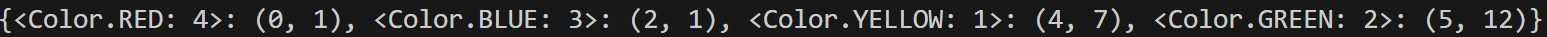
\includegraphics[width=1\textwidth]{dict_pos.png}  
  \caption{Dictionnaire position\_robot} 
  \label{fig:Dict}  
\end{figure}\\\\\\\\\\\\\\\
Ensuite pour résoudre le point (2) nous avons créé un tableau statique (\textit{\textbf{voir Améliorations de l'implémentation}}) de missions sous cette forme.
\begin{figure}[htbp]
  \centering  
  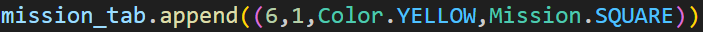
\includegraphics[width=0.5\textwidth]{mission.png}  
  \caption{Tableau de missions} 
  \label{fig:Mission}  
\end{figure}\\
Ainsi lorsque l'on initialise la grille on peut remplacer ses attibuts goal\_coordinate et color\_goal par les élements du tableau statique de mission. En tirant aléatoirement une position dans le tableau.\\\\
Les points (1) et (4) ont été les plus délicats. Ils impliquent une multitudes de méthodes de la classe "grid".\\\\ Le but était d'avoir une méthode qui initialisait un dictionnaire qui avait pour clefs la couleur de chaque robot et pour valeur une liste de dictionnaire de case atteignable avec pour clefs la direction et pour valeur la coordonnées de la case. Si cela vous parait trop compliqué voici un exemple.
\begin{figure}[htbp]
  \centering  
  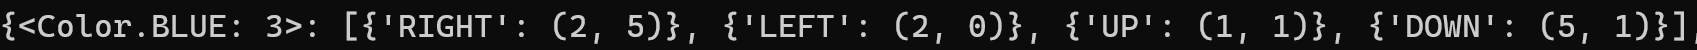
\includegraphics[width=0.9\textwidth]{possible_move.png}  
  \caption{Mouvements possibles par robot} 
  \label{fig:Mission}  
\end{figure}\\
Pour arriver à ce résultat il faut actualiser la position des robots dans la grille grâce à la méthode actualize\_robot\_position() et ensuite il faut voir sur les 4 directions (UP, RIGHT, DOWN, LEFT) quelles chemins peut emprunter le robot.\\\\ 
Pour cela on se sert de deux informations. La première c'est que le robot avance jusqu'à ce qu'il croise un mur. Pour cette condition il suffit de regarder l'attribut "wall" de la classe "Case" qui est un tableau de 4 booléens représentant la présence ou non de mur respectivement dans les 4 directions à une case donnée de la grille.\\\\
Ainsi si le robot veut aller en haut, il suffit de le faire avancer jusqu'à ce que la case sur laquelle il est, contient un mur dans la direction "UP" du tableau de booléen "wall". Il suffit de vérifier  " wall[0] == True ? Stop : Continue ".\\\\
La deuxième information est la suivante. Un robot peut arrêter sa progression si il croise un autre robot sur son chemin.\\\\ Cette condtion est assez simple à verifier si on se sert du dictionnaire position\_robot. On fait avancer le robot dans une direction en vérifiant à la n-ième "case + 1" qu'un autre robot ne s'y trouve pas. Si c'est le cas, on s'arrête, sinon on continue. 
\subsection{Problème de planification et de décision séquentiel}
Pour résoudre ce problème, il a fallu définir la représentation \textbf{d'un état} qui permettait d'illustrer l'entièreté de notre problème à un instant donné.\\\\ 
Grâce à notre travail préliminaire, un état à l'instant t sera représenté par le dictionnaire vu à la figure 4. Il ne faut pas oublier que la position des robots ne vaut rien sans la grille correspondante. \\\\
Ensuite il faut que l'on définisse \textbf{un système de production}. Pour cela, on se servira du dictionnaire vu à la figure 6.\\\\
Il faut ensuite définir un \textbf{état initial} et un ou des \textbf{état/s final/finaux}. Pour cela il suffit de prendre la position de départ de chaque robot (figure 4) pour l'état initial.\\\\
Pour les états finaux il suffit que la robot de la couleur de la mission soit sur les coordonnées de celle-ci et ça peut importe où se trouve les autres robots.\\\\
Une fois tout ce travail effectué, il faut maintenant appliquer \textbf{des stratégies de résolutions}.

\end{document}
